% ============================================================
% 1.6. Результаты исследования
% ============================================================
\subsection{Результаты исследования}

\subsubsection{Реализованная платформа}

В результате выполнения работы разработана платформа SopromatLab --- интерактивное веб-приложение для обучения основам сопротивления материалов. Платформа состоит из четырёх основных страниц, доступных через навигационное меню.

\textbf{Страница <<Калькулятор>>} (рис.~\ref{fig:calculator}) является центральным элементом платформы и обеспечивает:
\begin{itemize}
  \item выбор типа конструкции (консольная, шарнирно-опёртая, с вылетом);
  \item задание геометрических параметров (длина пролёта, длина вылета);
  \item управление нагрузками (добавление, редактирование, удаление сосредоточенных сил, распределённых нагрузок и моментов);
  \item выбор материала (сталь, алюминий, дерево) или ввод произвольных $E$ и $I$;
  \item мгновенное отображение эпюр $M(x)$, $Q(x)$, $N(x)$ и деформированной формы;
  \item интерактивный hover с отображением значений в любой точке;
  \item панель реакций опор с численными значениями;
  \item пошаговое решение задачи;
  \item панель верификации по Журавскому;
  \item контекстные подсказки.
\end{itemize}

\begin{figure}[H]
  \centering
  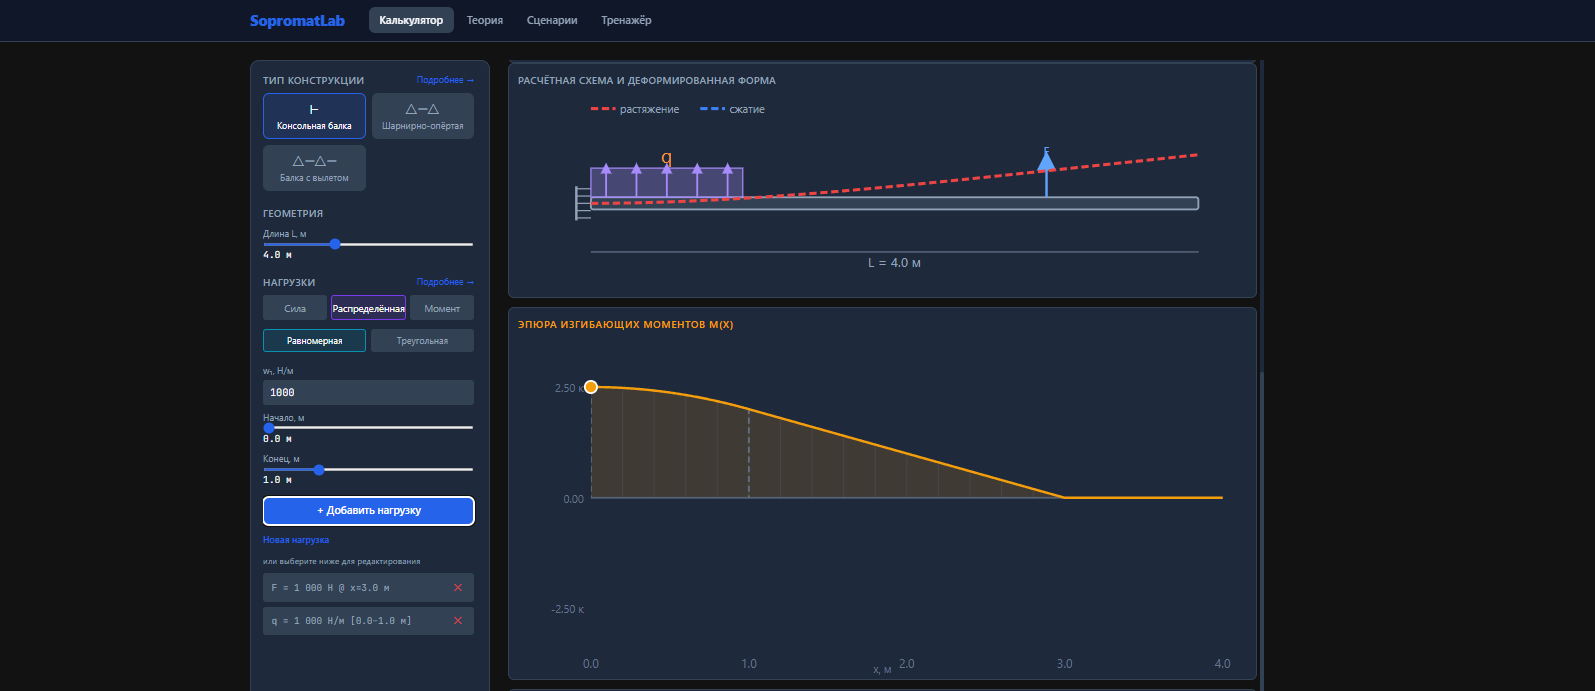
\includegraphics[width=0.95\textwidth]{images/beam_scheme.png}
  \caption{Основной интерфейс калькулятора балок с редактором и эпюрами}\label{fig:calculator}
\end{figure}

\begin{figure}[H]
  \centering
  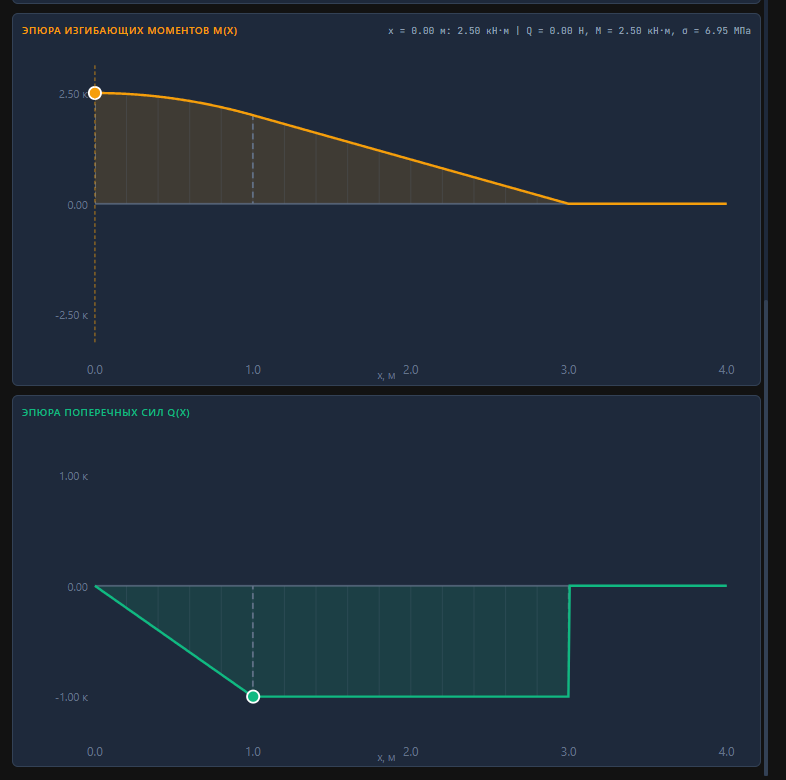
\includegraphics[width=0.95\textwidth]{images/diagrams_M_Q_N.png}
  \caption{Эпюры поперечных сил~$Q(x)$, изгибающих моментов~$M(x)$ и продольных сил~$N(x)$}\label{fig:diagrams}
\end{figure}

\begin{figure}[H]
  \centering
  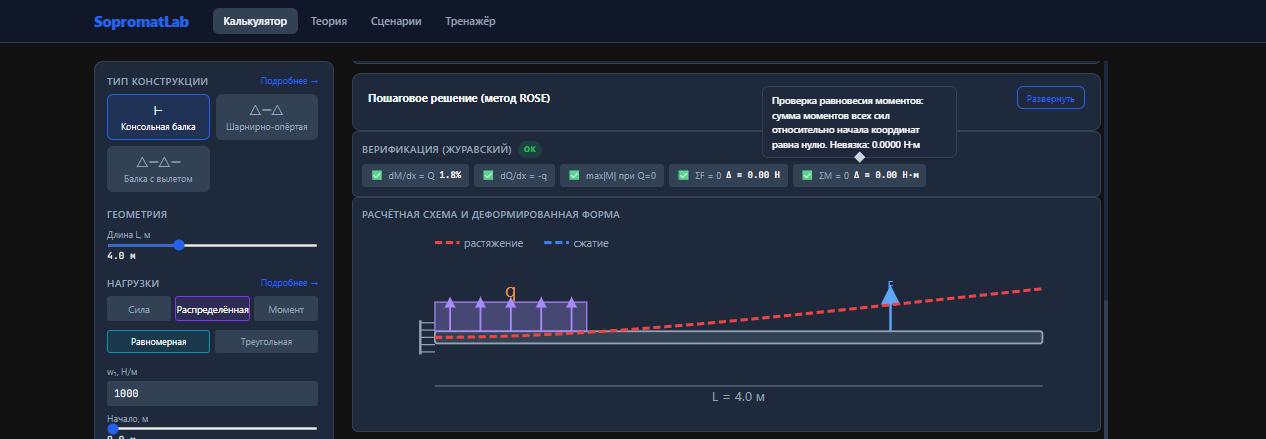
\includegraphics[width=0.9\textwidth]{images/verification_panel.png}
  \caption{Панель верификации результатов по зависимостям Журавского}\label{fig:verification}
\end{figure}

\textbf{Страница <<Теория>>} содержит 9~образовательных разделов с формулами, рендерируемыми через MathJax:
\begin{enumerate}
  \item Расчётные схемы балок --- типы, особенности, граничные условия.
  \item Сосредоточенные нагрузки --- скачки $Q$, изломы $M$, формулы.
  \item Распределённые нагрузки --- интегрирование, связь $Q$ и $M$.
  \item Сосредоточенные моменты --- скачки $M$, отсутствие влияния на $Q$.
  \item Материалы и модуль упругости --- $E$, $I$, жёсткость $EI$.
  \item Правила знаков --- определения $Q$, $M$, $N$, типичные ошибки.
  \item Дифференциальные зависимости Журавского --- $dQ/dx$, $dM/dx$, контрольные правила.
  \item Типичные ошибки --- систематизация 5~групп ошибок студентов.
  \item Прогибы и угол поворота --- дифференциальное уравнение, граничные условия.
\end{enumerate}

Каждый раздел содержит кнопку <<Попробовать в калькуляторе>>, которая загружает соответствующий пример в калькулятор для практического закрепления. Внешний вид страницы <<Теория>> показан на рис.~\ref{fig:theory}.

\begin{figure}[H]
  \centering
  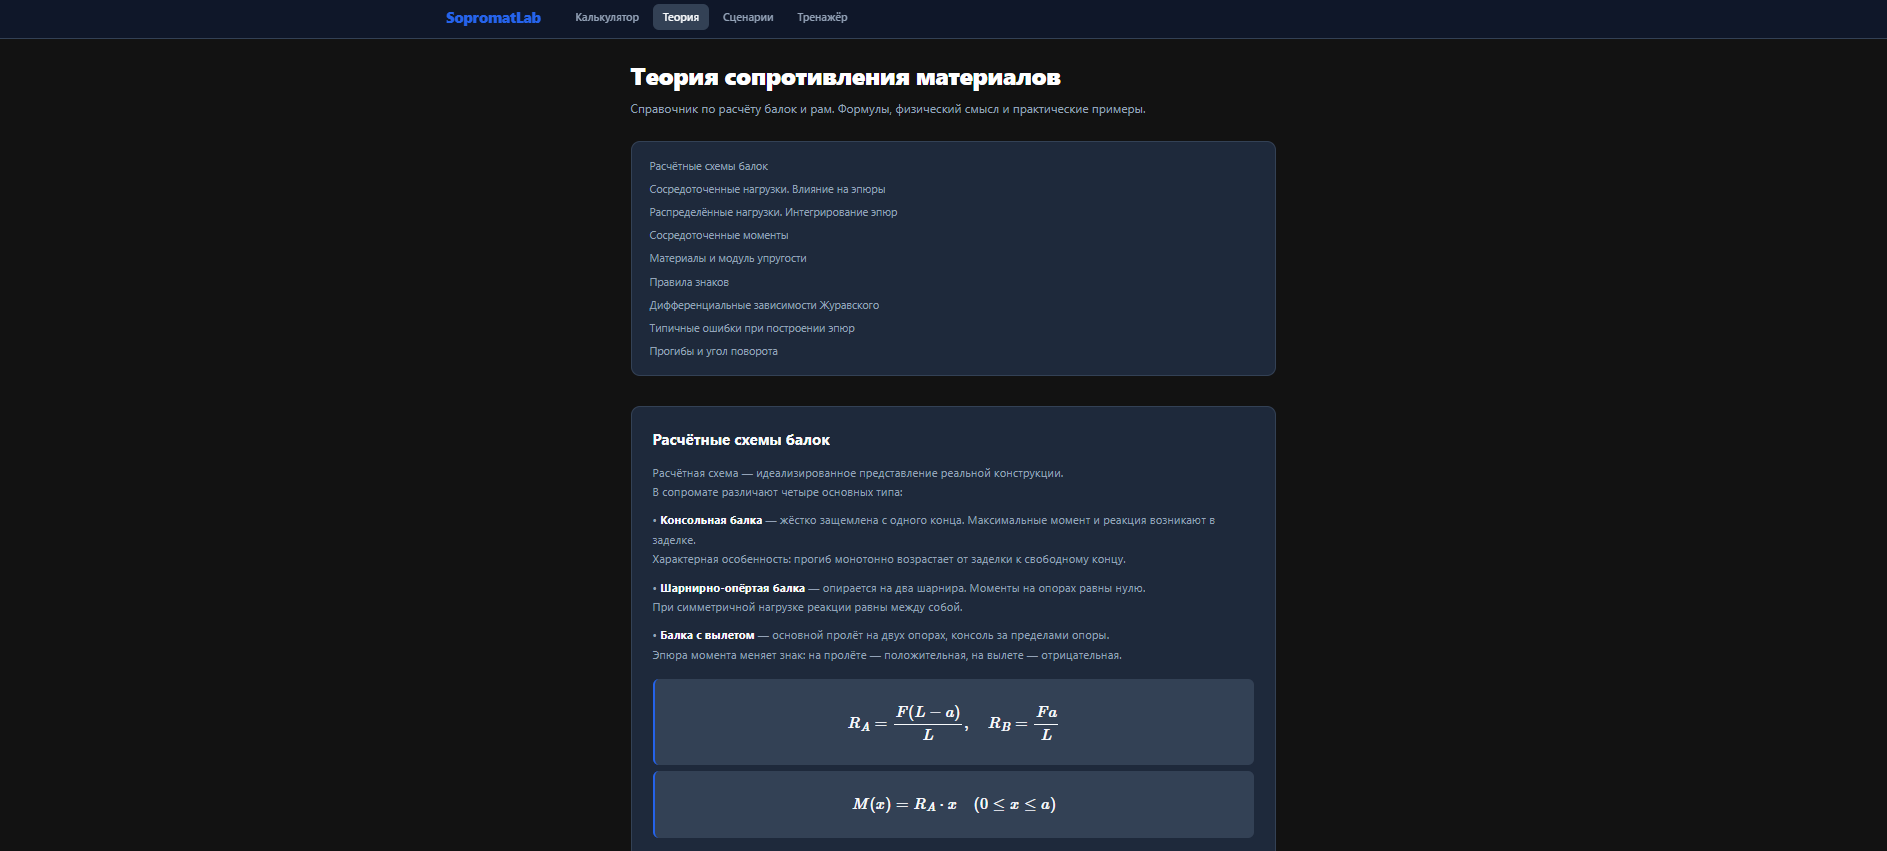
\includegraphics[width=0.9\textwidth]{images/theory.png}
  \caption{Страница <<Теория>> с образовательными разделами}\label{fig:theory}
\end{figure}

\textbf{Страница <<Сценарии>>} (рис.~\ref{fig:scenarios}) предлагает 5~готовых учебных задач, приближенных к реальным инженерным ситуациям (таблица~\ref{tab:scenarios}).

\begin{figure}[H]
  \centering
  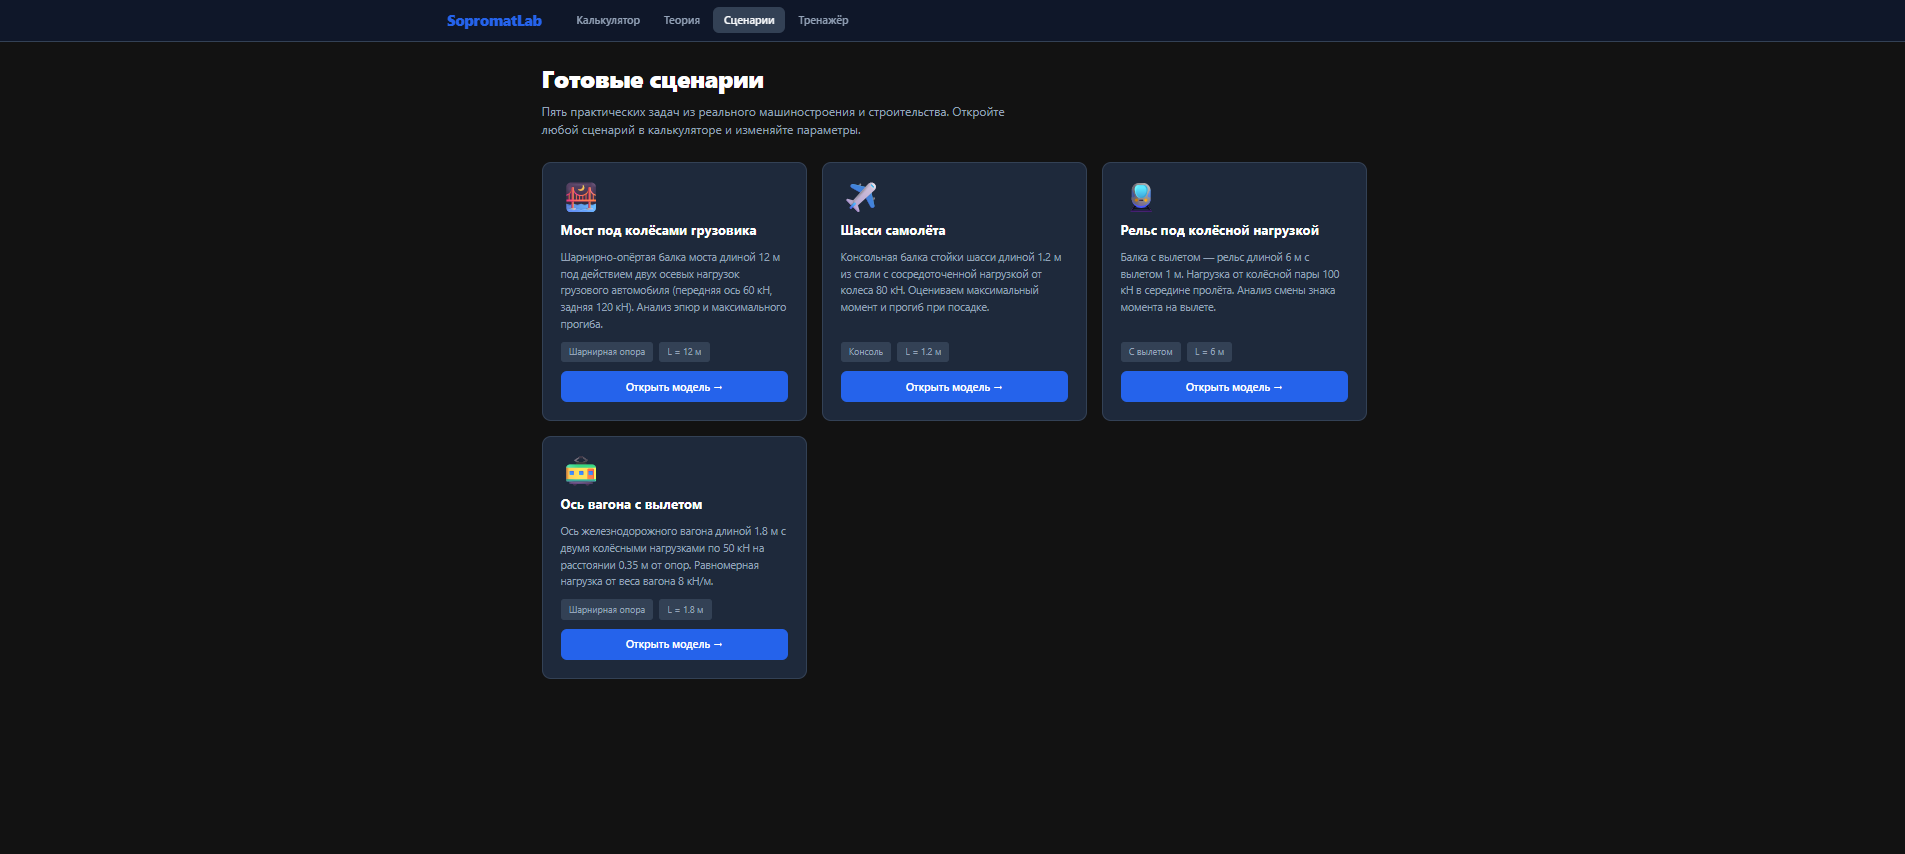
\includegraphics[width=0.9\textwidth]{images/scenarios.png}
  \caption{Страница <<Сценарии>> с учебными задачами}\label{fig:scenarios}
\end{figure}

\begin{table}[H]
\caption{Учебные сценарии платформы}\label{tab:scenarios}
\small
\begin{tabularx}{\textwidth}{|c|p{3cm}|l|c|X|}
\hline
\textbf{\#} & \textbf{Название} & \textbf{Тип} & \textbf{$L$, м} & \textbf{Нагрузки} \\
\hline
1 & Мост под грузовиком & Шарн.-опёрт. & 12 & $F_1 = 60$~кН ($a = 3$~м), $F_2 = 120$~кН ($a = 7$~м) \\
\hline
2 & Шасси самолёта & Консоль & 1,2 & $F = 80$~кН (свободный конец) \\
\hline
3 & Рельс & С вылетом & 6+1 & $F = 100$~кН ($a = 3$~м) \\
\hline
4 & Кронштейн двигателя & Консоль & 0,8 & $F = 5$~кН (горизонтальная) \\
\hline
5 & Ось вагона & Шарн.-опёрт. & 1,8 & $2 \times 50$~кН + $q = 8$~кН/м \\
\hline
\end{tabularx}
\end{table}

\textbf{Страница <<Тренажёр>>} (рис.~\ref{fig:trainer}) реализует режим самостоятельной проверки знаний:
\begin{itemize}
  \item генерация случайных задач: $L = 3\text{--}8$~м, 1--2~нагрузки (силы $1\text{--}20$~кН или $q = 2\text{--}15$~кН/м);
  \item ввод ответов студентом: $R_A$ (или $R_{\text{зад}}$), $R_B$ (или $M_{\text{зад}}$), $M_{\max}$, $Q_{\max}$;
  \item автоматическая проверка с допуском 5\%;
  \item цветовая индикация: зелёная рамка --- верно, красная --- ошибка;
  \item отображение правильных ответов и подсказки с методом решения после проверки.
\end{itemize}

\begin{figure}[H]
  \centering
  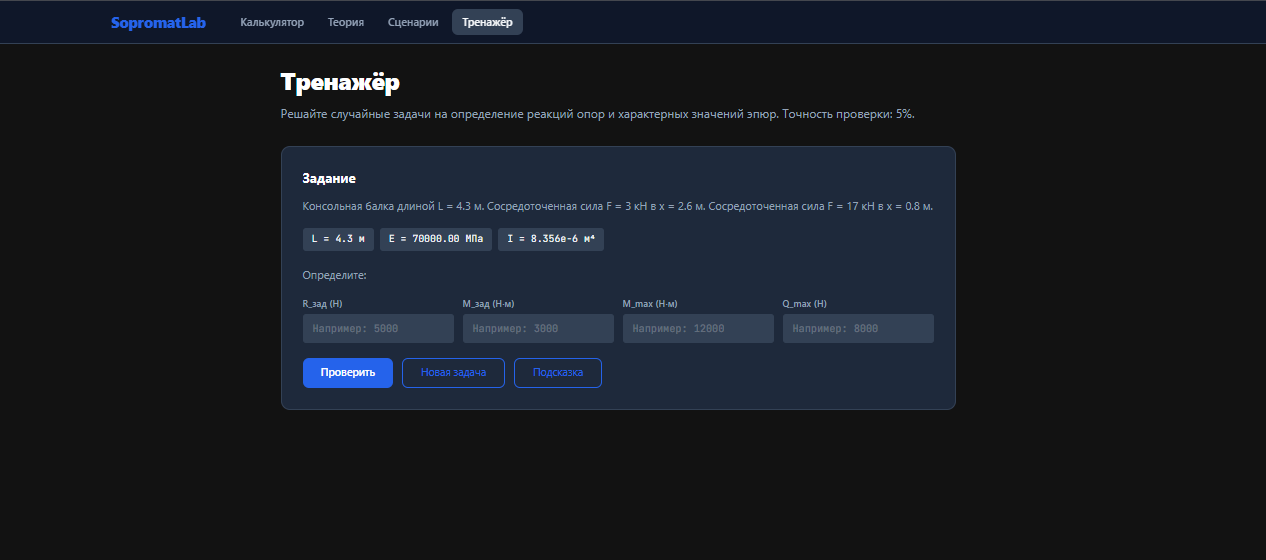
\includegraphics[width=0.9\textwidth]{images/trainer.png}
  \caption{Страница <<Тренажёр>> с режимом самопроверки}\label{fig:trainer}
\end{figure}

\subsubsection{Пошаговое решение}

Виджет \texttt{StepByStep} (рис.~\ref{fig:stepbystep}) реализует сворачиваемую панель, демонстрирующую 6~шагов решения задачи:
\begin{enumerate}
  \item \textbf{Расчётная схема} --- тип балки, параметры, $EI$.
  \item \textbf{Внешние нагрузки} --- перечисление всех нагрузок с параметрами.
  \item \textbf{Опорные реакции} --- формулы определения и численные значения.
  \item \textbf{Метод сечений ROSE} --- описание алгоритма, разбиение на участки.
  \item \textbf{Характерные значения} --- $Q_{\max}$, $M_{\max}$, $v_{\max}$ и их положения.
  \item \textbf{Деформации} --- дифференциальное уравнение, граничные условия, результат.
\end{enumerate}

\begin{figure}[H]
  \centering
  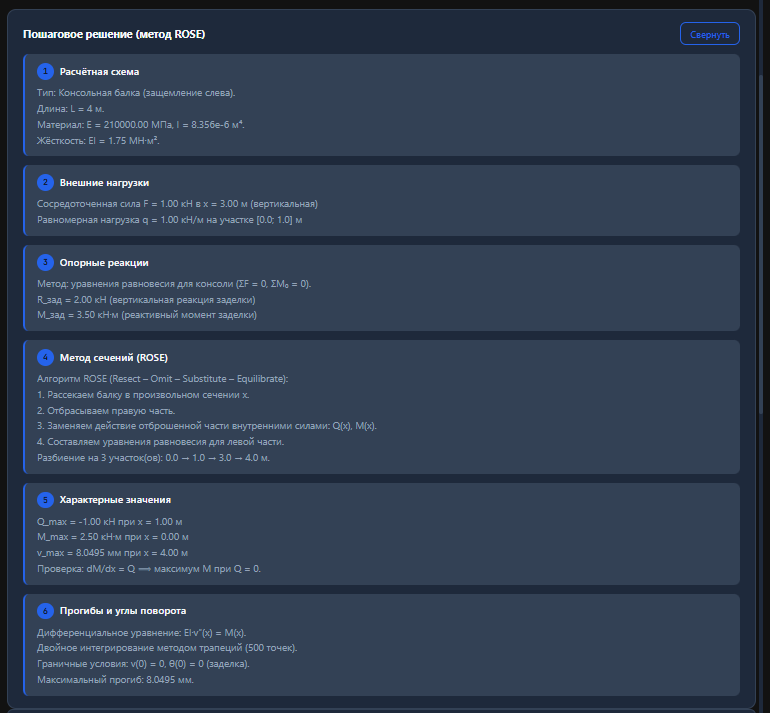
\includegraphics[width=0.9\textwidth]{images/step_by_step.png}
  \caption{Виджет пошагового решения задачи}\label{fig:stepbystep}
\end{figure}

Данный виджет позволяет студенту сопоставить свой ход решения с алгоритмом платформы и выявить источник ошибки.

\subsubsection{AI-консультант на базе большой языковой модели}

Для оказания индивидуальной помощи студенту в платформе реализован контекстный AI-консультант на базе большой языковой модели (LLM). Виджет \texttt{ChatAssistant} вызывается плавающей кнопкой в правом нижнем углу страницы калькулятора и открывает диалоговое окно, в котором студент может задать произвольный вопрос о текущей расчётной задаче на естественном языке.

Архитектура и принцип работы подсистемы подробно описаны в подразделе~\ref{sec:llm}. Ключевая особенность реализации --- передача модели текстового представления текущей конфигурации балки и результатов расчёта в составе системного промпта (подход~\textit{retrieval-augmented generation}). Благодаря этому модель отвечает на вопросы с привязкой к конкретным числовым значениям, отображённым в данный момент на экране, а не абстрактно.

Типичные сценарии использования:
\begin{itemize}
  \item <<Объясни, почему максимальный момент возникает именно в этой точке>> --- модель связывает положение экстремума с условием $Q(x_0) = 0$ и подставляет конкретные значения координат и нагрузок;
  \item <<Что произойдёт, если уменьшить момент инерции в~2~раза?>> --- модель применяет известную обратную пропорциональность $v \sim 1/I$ и даёт численную оценку нового прогиба;
  \item <<Безопасна ли такая балка для стали с допускаемым напряжением 160~МПа?>> --- модель вычисляет $\sigma_{\max} = M_{\max} / W$ и сравнивает с допускаемым;
  \item <<Почему верификация по Журавскому не пройдена?>> --- модель анализирует сообщение и подсказывает возможные причины (ошибка в нагрузке, неправильно заданная опора).
\end{itemize}

Серверная часть AI-консультанта реализована на Node.js + Express и обращается к API провайдера OpenRouter, что обеспечивает гибкость выбора модели (GPT, Claude, Llama, DeepSeek и др.) без изменения клиентского кода. Такая архитектура позволяет легко переключаться между моделями в зависимости от доступности и стоимости. История диалога ограничена последними~10 сообщениями, что обеспечивает разумную стоимость запроса при сохранении контекста разговора. Применение LLM в образовательном контексте соответствует современным исследованиям~\cite{kasneci2023chatgpt}, согласно которым контекстно-связанные диалоговые модели существенно повышают вовлечённость студентов и помогают преодолевать <<тупиковые состояния>>, в которые они попадают при самостоятельной работе.

\subsubsection{Контекстные подсказки}

Система контекстных подсказок включает 21~условие, классифицированных по трём группам:

\textbf{Физические закономерности:}
\begin{itemize}
  \item симметрия нагрузки $\Rightarrow$ симметрия эпюры $M$ и антисимметрия $Q$;
  \item $Q(x_0) = 0$ $\Rightarrow$ экстремум $M(x_0)$;
  \item от $q = \text{const}$: $Q$ --- линейная, $M$ --- параболическая;
  \item при увеличении $L$ прогиб растёт как $L^3$ (для сосредоточенной силы).
\end{itemize}

\textbf{Конструктивные особенности:}
\begin{itemize}
  \item смена знака $M$ на вылете балки;
  \item $R_A < 0$ при доминировании нагрузки на вылете.
\end{itemize}

\textbf{Предупреждения:}
\begin{itemize}
  \item отсутствие нагрузок;
  \item нагрузка, совпадающая с опорой;
  \item чрезмерный прогиб ($v_{\max} > L/200$);
  \item верификация не пройдена;
  \item малая жёсткость $EI$;
  \item высокая нагрузка.
\end{itemize}

\subsubsection{Экспорт и обмен}

\textbf{Share-ссылка.} Конфигурация балки (\texttt{BeamConfig}) сериализуется в JSON и кодируется в Base64. Результат передаётся через URL-параметр \texttt{?c=...}. При открытии ссылки конфигурация автоматически восстанавливается, что позволяет преподавателю передать задачу студенту или студенту --- поделиться решением.

\textbf{PDF-отчёт.} Генерируется документ формата A4 (альбомная ориентация), содержащий:
\begin{itemize}
  \item заголовок и дату формирования;
  \item скриншот эпюр и расчётной схемы (через html2canvas с масштабом $\times 2$);
  \item таблицу характерных значений ($L$, $E$, $I$, $Q_{\max}$, $M_{\max}$, $v_{\max}$);
  \item реакции опор;
  \item результат верификации по Журавскому (статус, RMS-ошибка, невязки равновесия).
\end{itemize}

\subsubsection{Подробные верификационные примеры}

Для подтверждения корректности расчётного ядра платформы SopromatLab были выполнены контрольные расчёты четырёх классических задач сопротивления материалов, для которых известны точные аналитические решения~\cite{feodosev, timoshenko, gere2018}. В каждом примере приведено ручное (аналитическое) решение, после чего результат сравнивается с числовым ответом, полученным платформой.

\textit{Пример~1. Консольная балка с сосредоточенной силой на свободном конце.}

Дано: $L = 2$~м, $E = 2{,}1 \cdot 10^{11}$~Па (сталь), $I = 8 \cdot 10^{-6}$~м$^4$, $F = 10$~кН на свободном конце ($x = L$). Опора (заделка) расположена в точке~$A$ ($x = 0$).

Аналитическое решение. Из уравнений равновесия отделённой части балки находим реакции в заделке:
\begin{equation}
  R_A = F = 10\text{ кН}, \qquad M_A = -F \cdot L = -10 \cdot 2 = -20 \text{ кН$\cdot$м}.
  \label{eq:ex1_reactions}
\end{equation}

Внутренние силовые факторы в произвольном сечении $x$ определяются по правилу метода сечений (рассматриваем правую часть):
\begin{equation}
  Q(x) = F = 10 \text{ кН}, \qquad M(x) = -F \cdot (L - x) = -10 \cdot (2 - x).
  \label{eq:ex1_QM}
\end{equation}

Максимальный изгибающий момент по модулю $|M_{\max}| = 20$~кН$\cdot$м возникает в заделке. Прогиб свободного конца получается из классической формулы~\cite{feodosev}:
\begin{equation}
  v_{\max} = \frac{F L^3}{3 E I} = \frac{10000 \cdot 2^3}{3 \cdot 2{,}1 \cdot 10^{11} \cdot 8 \cdot 10^{-6}} \approx 1{,}587 \cdot 10^{-2} \text{ м} \approx 15{,}87 \text{ мм}.
  \label{eq:ex1_vmax}
\end{equation}

Результат платформы для этой же конфигурации: $R_A = 10{,}000$~кН, $M_A = -20{,}000$~кН$\cdot$м, $|M_{\max}| = 20{,}000$~кН$\cdot$м, $v_{\max} = 15{,}873$~мм. Относительное отклонение прогиба от аналитического значения: $\delta = |15{,}873 - 15{,}87| / 15{,}87 \approx 0{,}02\%$, что значительно ниже принятого порога допуска в~5\%.

\textit{Пример~2. Шарнирно-опёртая балка с сосредоточенной силой в середине пролёта.}

Дано: $L = 4$~м, $E = 2{,}1 \cdot 10^{11}$~Па, $I = 1{,}2 \cdot 10^{-5}$~м$^4$, $F = 20$~кН в точке $x = L/2 = 2$~м.

Аналитическое решение. Из условий равновесия (симметрия): $R_A = R_B = F/2 = 10$~кН. На участке $0 \leq x \leq L/2$:
\begin{equation}
  Q(x) = R_A = 10 \text{ кН}, \qquad M(x) = R_A \cdot x = 10 x.
  \label{eq:ex2_left}
\end{equation}

В точке приложения силы момент достигает максимума:
\begin{equation}
  M_{\max} = M(L/2) = R_A \cdot L/2 = \frac{F L}{4} = \frac{20 \cdot 4}{4} = 20 \text{ кН$\cdot$м}.
  \label{eq:ex2_Mmax}
\end{equation}

Прогиб в середине пролёта~\cite{gere2018}:
\begin{equation}
  v_{\max} = \frac{F L^3}{48 E I} = \frac{20000 \cdot 4^3}{48 \cdot 2{,}1 \cdot 10^{11} \cdot 1{,}2 \cdot 10^{-5}} \approx 1{,}058 \cdot 10^{-2} \text{ м} \approx 10{,}58 \text{ мм}.
  \label{eq:ex2_vmax}
\end{equation}

Результат платформы: $R_A = R_B = 10{,}000$~кН, $M_{\max} = 20{,}000$~кН$\cdot$м (при $x = 2{,}0$~м), $v_{\max} = 10{,}585$~мм (при $x = 2{,}0$~м). Отклонение: $\delta \approx 0{,}05\%$. Эпюра $M(x)$ имеет характерный треугольный вид с изломом в точке приложения силы; эпюра $Q(x)$ --- ступенчатый скачок на $-F$ при $x = L/2$, что соответствует физической природе сосредоточенной силы.

\textit{Пример~3. Шарнирно-опёртая балка с равномерно распределённой нагрузкой.}

Дано: $L = 6$~м, $E = 2{,}1 \cdot 10^{11}$~Па, $I = 2 \cdot 10^{-5}$~м$^4$, $q = 5$~кН/м, действующая по всей длине пролёта.

Аналитическое решение. Реакции опор по симметрии: $R_A = R_B = q L / 2 = 15$~кН. Поперечная сила и изгибающий момент:
\begin{equation}
  Q(x) = R_A - q x = 15 - 5 x, \qquad M(x) = R_A x - \frac{q x^2}{2} = 15 x - 2{,}5 x^2.
  \label{eq:ex3_QM}
\end{equation}

Максимум момента находится из условия $Q(x_0) = 0$, откуда $x_0 = L/2 = 3$~м, и:
\begin{equation}
  M_{\max} = \frac{q L^2}{8} = \frac{5 \cdot 36}{8} = 22{,}5 \text{ кН$\cdot$м}.
  \label{eq:ex3_Mmax}
\end{equation}

Прогиб в середине пролёта по классической формуле~\cite{feodosev}:
\begin{equation}
  v_{\max} = \frac{5 q L^4}{384 E I} = \frac{5 \cdot 5000 \cdot 6^4}{384 \cdot 2{,}1 \cdot 10^{11} \cdot 2 \cdot 10^{-5}} \approx 2{,}009 \cdot 10^{-2} \text{ м} \approx 20{,}09 \text{ мм}.
  \label{eq:ex3_vmax}
\end{equation}

Результат платформы: $R_A = R_B = 15{,}000$~кН, $M_{\max} = 22{,}500$~кН$\cdot$м, $v_{\max} = 20{,}089$~мм. Отклонение прогиба: $\delta \approx 0{,}05\%$. Эпюра $M(x)$ имеет вид параболы с вершиной в середине пролёта; эпюра $Q(x)$ --- линейная функция, проходящая через ноль в точке экстремума момента, что подтверждает выполнение зависимости Журавского $dM/dx = Q$.

\textit{Пример~4. Консольная балка с равномерно распределённой нагрузкой.}

Дано: $L = 3$~м, $E = 7 \cdot 10^{10}$~Па (алюминий), $I = 5 \cdot 10^{-6}$~м$^4$, $q = 4$~кН/м, действующая по всей длине балки. Заделка в точке $A$ ($x = 0$).

Аналитическое решение. Полная реакция заделки --- вертикальная сила $R_A = q L = 12$~кН и реактивный момент:
\begin{equation}
  M_A = -\frac{q L^2}{2} = -\frac{4 \cdot 9}{2} = -18 \text{ кН$\cdot$м}.
  \label{eq:ex4_reactions}
\end{equation}

Поперечная сила и момент в произвольном сечении (рассматриваем левую часть):
\begin{equation}
  Q(x) = R_A - q x = 12 - 4 x, \qquad M(x) = M_A + R_A x - \frac{q x^2}{2} = -18 + 12 x - 2 x^2.
  \label{eq:ex4_QM}
\end{equation}

Максимальный по модулю момент возникает в заделке: $|M_{\max}| = 18$~кН$\cdot$м. Прогиб свободного конца~\cite{gere2018}:
\begin{equation}
  v_{\max} = \frac{q L^4}{8 E I} = \frac{4000 \cdot 3^4}{8 \cdot 7 \cdot 10^{10} \cdot 5 \cdot 10^{-6}} \approx 1{,}157 \cdot 10^{-1} \text{ м} \approx 115{,}71 \text{ мм}.
  \label{eq:ex4_vmax}
\end{equation}

Результат платформы: $R_A = 12{,}000$~кН, $M_A = -18{,}000$~кН$\cdot$м, $v_{\max} = 115{,}74$~мм. Отклонение: $\delta \approx 0{,}03\%$. Поскольку в данном расчёте прогиб превышает $L/200 = 15$~мм, контекстная подсказка платформы автоматически выдаёт предупреждение о чрезмерной деформации и рекомендует увеличить жёсткость сечения, что демонстрирует работу образовательной обратной связи.

Максимальное наблюдаемое отклонение численного решения от аналитического по всем четырём примерам составило менее~0{,}1\%, что на порядок ниже принятого порога допуска. Автоматическая верификация по зависимостям Журавского во всех случаях даёт нормированную RMS-ошибку менее~$10^{-3}$, что согласуется с теоретической оценкой $O(h^2)$ метода трапеций при $N = 500$. Верификационные примеры охватывают все основные комбинации нагрузок и опор и подтверждают корректность расчётного ядра в полном диапазоне поддерживаемых задач.

\subsubsection{Производительность}

Замеры времени расчёта проведены в браузере Google Chrome на процессоре средней мощности:
\begin{itemize}
  \item расчёт одной конфигурации (500~точек, 3~нагрузки): $< 5$~мс;
  \item рендеринг SVG-эпюр: $< 16$~мс (60~fps);
  \item генерация PDF-отчёта: $\sim 2$~с (включая захват экрана).
\end{itemize}

Суммарное время от изменения параметра до обновления визуализации составляет менее~20~мс, что обеспечивает восприятие пересчёта как <<мгновенного>> (порог восприятия задержки составляет~100~мс)~\cite{flanagan2020}.

\subsubsection{Ключевые метрики платформы}

По результатам разработки платформа SopromatLab характеризуется следующими количественными показателями (таблица~\ref{tab:metrics}).

\begin{table}[H]
\caption{Ключевые метрики платформы SopromatLab}\label{tab:metrics}
\begin{tabularx}{\textwidth}{|X|c|}
\hline
\textbf{Параметр} & \textbf{Значение} \\
\hline
Типов балок & 3 \\
\hline
Типов нагрузок & 3 (с 2 вариантами распределённой) \\
\hline
Материалов-пресетов & 3 + кастомный \\
\hline
Точек дискретизации & 500 \\
\hline
Разделов теории & 9 \\
\hline
Контекстных подсказок & 21 \\
\hline
Готовых учебных сценариев & 5 \\
\hline
Шагов пошагового решения & 6 \\
\hline
Погрешность прогибов & $< 0{,}5\%$ \\
\hline
Время расчёта & $< 5$~мс \\
\hline
Объём кода (TypeScript/TSX) & $\sim 1500$~строк \\
\hline
\end{tabularx}
\end{table}

Платформа поддерживает несколько режимов учебного применения: самостоятельную работу студента с готовыми сценариями и собственными конфигурациями; подготовку к практическим занятиям в качестве средства быстрой проверки ручных расчётов; лекционные демонстрации зависимостей $v \sim L^3$ и $v \sim 1/EI$ в реальном времени; тренажёр с автоматической проверкой; обмен заданиями между преподавателем и студентами через Share-ссылку. По сравнению с существующими аналогами (MDSolids~\cite{philpot2003}, SkyCiv, StructLab~\cite{vasilenko}) платформа сочетает преимущества веб-доступа без установки с расширенными образовательными функциями (пошаговое решение, контекстные подсказки, тренажёр, автоматическая верификация по зависимостям Журавского), часть из которых отсутствует у всех рассмотренных аналогов.
